\documentclass[oneside]{scrbook}			%
\usepackage[english]{babel}
\usepackage[pdftex]{graphicx} 	% Einbinden von Bildern
\usepackage{tabularx}
\usepackage{float}			%H in grafiken
\usepackage{amssymb}
\usepackage[left=2.5cm, right=2.5cm, bottom=2.5cm, top=2cm]{geometry}
\usepackage{verbatim}
\usepackage{lipsum}
\usepackage{siunitx} % SI_UNITS https://www.dickimaw-books.com/latex/thesis/html/siunitx.html
\usepackage{amsmath}
\usepackage{braket} %bra-ket notation
\usepackage{hyperref}
\usepackage{epstopdf}
\usepackage{graphicx}
\usepackage{capt-of}
\usepackage{tikz}
\usepackage[font=small,labelfont=bf,labelsep=space]{caption}
\usepackage[caption=false,font=footnotesize]{subfig}

%%%%%%%%%%%%%%%%%%%%%%%%%%%%%%%%%%%%%%%%%%%%%%%%%%%%%%%%
% DOC FORMAT SETTINGS
\setlength\parindent{0pt}
\captionsetup{figurename=Fig.,	tablename=Tab.	}
%%%%%%%%%%%%%%%%%%%%%%%%%%%%%%%%%%%%%%%%%%%%%%%%%%%%%%%%
% TIKZ SETTINGS
\usetikzlibrary{shapes.geometric,
                calc, %for relative coord calculations
                decorations.pathmorphing, %for snake lines
                decorations.pathreplacing, %for braces
                shapes,
                arrows.meta, % for double arrow
                backgrounds,
                positioning} % for position along lines
%%%%%%%%%%%%%%%%%%%%%%%%%%%%%%%%%%%%%%%%%%%%%%%%%%%%%%%%
% Custom functions

\newcommand{\gtlt}{% greater than less than
{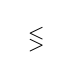
\begin{tikzpicture}%
\node[inner sep=0, outer sep=0] at (0,0) {$\scriptstyle <$};
\node[inner sep=0, outer sep=0] at (0,-0.15) {$\scriptstyle >$};
\end{tikzpicture}%
}}








%%%%%%%%%%%%%%%%%%%%%%%%%%%%%%%%%%%%%%%%%%%%%%%%%%%%%%%%
\begin{document}
\begin{titlepage}
\begin{center}
  \includegraphics[width=35mm]{./graph/TU_Signet.pdf} \\[10mm]
  {\LARGE \textsc{Bachelor Thesis:}}\\[10mm]
  {\LARGE Impact Ionisation in Quantum Dot - Benzene Heterostructures with non-local coulomb Interactions }\\[10mm]
  	Supervisors:\\
  Prof. Dr. Karsten Held,\\
  Projektass. Paul Worm, PhD\\
  \vspace{5mm}
  Institute of Solid State Physics\\
  Quantum many body physics group\\
  Technische Universit\"at Wien\\[5mm]
  
  by\\[5mm]
  \textbf{Benjamin Orthner}\\
  00473828
\end{center}
  \date{\today}
\vspace{\fill}
\begin{flushright} %\begin{bottompar} 
\makeatletter
\@date
\makeatother
\end{flushright}
\end{titlepage}


%\maketitle 
\thispagestyle{empty} \clearpage										% Deckblatt
\pagestyle{plain} \pagenumbering{Roman} %\tableofcontents 					% Verzeichnisse

\pagenumbering{arabic}
\counterwithout{footnote}{chapter}
% % % % % % % % % % % % % % % % % % % % % % % % % % % % % % % % % % % % % % % % % % % % % % % % % %
%\addcontentsline{toc}{section}{Abstract}

%   Reduce the margin:
\def\changemargin#1#2{\list{}{\rightmargin#2\leftmargin#1}\item[]}
\let\endchangemargin=\endlist 

% title
{\small\begin{center}%
\bfseries{Abstract}
\end{center}}

% Abstract
\begin{changemargin}{1cm}{1cm}

Solar power is one of the most promising low carbon energy technologies, allowing the generation of electricity from free and abundant sunlight. With ever increasing energy demands on top of the looming threat of a climate crisis, innovations in this field are essential. However, progress in conventional silicon-based solar cell technologies has begun to stagnate, as they approach their inherent maximum efficiency of $34\%$, the Shockley-Queisser-limit \cite{shockley_queisser}. Among a few other proposed alternatives, heterostructures of transition metal oxides may present a solution to this problem, as they display an effect called ``impact ionisation''.

\smallskip

This thesis builds upon previous works \cite{innerberger, worm_bachelor, prauhart, worm_project} which have implemented the Hubbard model to investigate impact ionisation in a small cluster of atoms within oxide heterostructures being excited by a short light pulse. We expand the capabilities of the existing code to include non-local coulomb interactions and set up the framework needed to allow the investigation of impact ionisation in a system consisting of a quantum dot coupled to a benzene ring. The Benzene Ring is modelled as a mono-atomic chain with periodic boundary conditions, and the non-local coulomb interactions are calculated via the Pariser-Parr-Pople method.

\smallskip
{\color{blue} rework second paragraph to include a mention of experimental paper using quantum dot benzene structure and non-local coulomb interactions being necessary to investigate this (especially for benzene)}
\end{changemargin}
\tableofcontents
\chapter{Introduction}
\section{Solar Cells}

Solar cells are devices that convert radiation energy into electrical energy via the photovoltaic effect. This is most commonly achieved using the doped semiconductor silicon. In order to understand how they work, we must first understand the electron structure of silicon.
\medskip

In a semiconductor, at $T=\SI{0}{\kelvin}$ all electrons occupy the so called valence band, which is separated from the unoccupied conductance band by an energy gap of $\sim \SI{1}{eV}$. One way for an electron to traverse this gap is by absorbing a photon with a energy higher than that of the band gap. This excitation of an electron into the conduction band leads to an increase in the electric current in the material. If the energy of the photon far exceeds that of the gap, the promoted electron bleeds off this excess energy in a process called thermalisation, in which phonons are excited and heat up the material. The excess energy is effectively lost. If the photon's energy is lower than that of the gap, it does not get absorbed at all. Because the sun radiates light on a spectrum, all solar cells  of this type are subject to an inherent limit in efficiency, the Shockley-Queisser-limit, which under ideal conditions can reach a maximum of about $34\%$ \cite{shockley_queisser}.

\medskip

Various methods do exist that have the potential to overcome this limit. Among these is an effect called ``impact ionisation''. To a small degree this effect occurs in most materials and allows for the excess energy of an excited electron to be used in the excitation of a second electron, instead of being lost to thermalisation. The factor deciding which of the two effects dominates, is the time-scale on which they occur. In semiconductors relaxation via phonon excitations occur on a time-scale of about $0.1 - 10 \si{\pico\second}$ where for impact ionisation it is about $1-100\si{\pico\second}$, thus making the former far more likely. However, in some materials with strongly correlated electron systems, such as oxide heterostructures, the time-scale for impact ionisation can be as low as $\SI{10}{\femto\second}$, thus making it the predominant process for electron relaxation \cite{time_scales}.


\colorlet{conductance}{black!7}
\colorlet{valence}{cyan!80!yellow!40}
\colorlet{cphoton}{yellow!70!red}
\colorlet{cphonon}{red!80!yellow}
\colorlet{cimpact}{cyan!70!red}


\begin{figure}[!hbt]
    \begin{minipage}[b]{.48\textwidth}
        \centering
        \begin{tikzpicture}[decoration=snake,
                        hole/.style={circle, draw, fill=white},
                        electron/.style={circle, draw, fill=cyan!80!yellow},
                        std_arrow/.style={->, >=Latex, thick},
                        photon/.style={->, thick, decorate, cphoton},
                        phonon/.style={->, thick, decorate, cphonon}
                        ]
            %%%%%%%%%%%%%%%%%%%%%
            % ELECTRONS & BANDS %
            %%%%%%%%%%%%%%%%%%%%%
            
            \newdimen \gap
            \newdimen \xshift
            \gap = 1.2cm
            \xshift = 1.1cm
            \draw[fill=valence] (0,0) rectangle (5, -1.5);
                \node[label={[valence!200]above right: Valence Band}, inner sep = 0.5] at (0, -1.5){};
            \draw[fill=conductance] (0, \gap) rectangle ($(5, 2.8) + (0,\gap)$);
                \node[label={[conductance!300]below right: Conduction Band}, inner sep = 0.5] at ($(0, 2.8) + (0, \gap)$){};
            \node[hole] at (\xshift,-0.3) (H){};
            \node[electron] at ($(H) + (0,3.5)$) (E1){};
            \node[electron] at ($(E1) + (1.3, -1.7)$) (E2){};
            
            %%%%%%%%%%%%%%%%%%
            % ARROWS N STUFF %
            %%%%%%%%%%%%%%%%%%
            
            \newdimen\phononlen
            \phononlen = 1.8cm
            \draw[photon] (0.05,0.4\gap) -- (\xshift, 0.4\gap) node[midway, above]{$\hbar\omega$};
            \draw[std_arrow] (H) -- (E1);
            \draw[std_arrow] (E1) -- (E2)
                node[pos=0.2](s1){}
                node[pos=0.4](s2){}
                node[pos=0.6](s3){};
            \foreach \i in {1,2,3}{
            \draw[phonon] ($(s\i) + (0.2, 0)$) -- ($(s\i) + (\phononlen,0)$);}
            \node[label=right:\color{cphonon}$\hbar \Omega$, inner sep = 0.2] at ($(s2) + (0.2, 0) + (\phononlen, 0)$){};
            
            \draw[->,>=Latex, ultra thick, black!20] (-0.5, -1.5) -- ($(-0.5, 3.3)+(0,\gap)$) node[right]{$E$};
        \end{tikzpicture}%
        \caption{After excitation by a photon, the excess energy of the electron is lost to thermalisation.\newline}
        \label{fig:thermalisation}
    \end{minipage}
    \hfill
    \begin{minipage}[b]{.48\textwidth}
        \centering
        \begin{tikzpicture}[hole/.style={circle, draw, fill=white},
                        electron/.style={circle, draw, fill=cyan!80!yellow},
                        std_arrow/.style={->, >=Latex, thick},
                        photon/.style={->, thick, decorate, decoration=snake, cphoton},
                        phonon/.style={->, thick, decorate, decoration=snake, cphonon},
                        impact_io/.style={->, thick, decorate, decoration=snake, cimpact},
                        brace/.style={decorate, decoration={brace, amplitude=6pt}, thick, color=gray}
                        ]
            %%%%%%%%%%%%%%%%%%%%%
            % ELECTRONS & BANDS %
            %%%%%%%%%%%%%%%%%%%%%
            
            \newdimen \gap
            \newdimen \xshift
            \gap = 1.2cm
            \xshift = 1.1cm
            \draw[fill=valence] (0,0) rectangle (5, -1.5);
                \node[label={[valence!200]above right: Valence Band}, inner sep = 0.5] at (0, -1.5){};
            \draw[fill=conductance] (0, \gap) rectangle ($(5, 2.8) + (0,\gap)$);
                \node[label={[conductance!300]below right: Conduction Band}, inner sep = 0.5] at ($(0, 2.8) + (0, \gap)$){};
            \node[hole] at (\xshift,-0.3) (H1){};
            \node[hole] at ($(H1) + (2.5,0)$) (H2) {};
            \node[electron] at ($(H) + (0,3.5)$) (E1){};
            \node[electron] at ($(E1) + (1.3, -1.7)$) (E2){};
            \node[electron] at ($(H2) + (0, \gap) + (0, 0.6)$) (E3){};
            
            %%%%%%%%%%%%%%%%%%
            % ARROWS N STUFF %
            %%%%%%%%%%%%%%%%%%
            
            \newdimen\phononlen
            \phononlen = 1.8cm
            \draw[photon] (0.05,0.4\gap) -- (\xshift, 0.4\gap) node[midway, above]{$\hbar\omega$};
            \draw[std_arrow] (H1) -- (E1);
            \draw[std_arrow] (E1) -- (E2) node[pos=0.43, inner sep=0] (E1_E2){};
            \draw[std_arrow] (H2) -- (E3) node[pos=0.5, inner sep=0] (H2_E3){};
            
            \draw[impact_io] (E1_E2) to[out=260,in=180] (H2_E3);
            
            \draw[->,>=Latex, ultra thick, black!20] (-0.5, -1.5) -- ($(-0.5, 3.3)+(0,\gap)$) node[right]{$E$};
            
            %%%%%%%%%%
            % Braces %
            %%%%%%%%%%
            \draw[brace] ($(E3.east) + (0.2,0)$) -- ($(H2.east) + (0.2,0)$) node[midway,right,xshift=.2cm] {$\Delta E_1$};
            \draw[brace] ($(E2.east) + (0.2,1.7)$) -- ($(E2.east) + (0.2,0)$) node[midway, right, xshift=.2cm] {$\Delta E_1$};
        \end{tikzpicture}
        \caption{After excitation by a photon, the excess energy is used  to excite a second electron to the conduction band via impact ionisation.}
        \label{fig:impact_ionisation}
    \end{minipage}
\end{figure}



\section{Existing Implementation}
In order to study the effects of impact ionisation in solar cells by means of small Hubbard clusters a program was developed. The original numerical implementation was by Michael Innerberger \cite{innerberger} and extensions were carried out by Paul Worm \cite{worm_bachelor, worm_project} and Paul Prauhart \cite{prauhart}.
\medskip

In this section we will only give a brief overview of the main functionality of the code and refer the reader back to the previously mentioned three papers for more details.

\subsection{Hubbard Model} \label{sec:hubbard_model}
To study the effect of impact ionisation in strongly correlated electron system the Hubbard model was used. It describes system of atoms as a lattice of $N_s\in \mathbb{N}$ sites, each of which can represent the location of at most one spin-up electron and one spin-down electron under the tight-binding approximation. The wave functions that describe such localised electrons are called Wannier-Functions.
\medskip

Using the second quantisation formalism of quantum mechanics, states of such many-body systems can be described purely by the occupation numbers of each site $n_{i\sigma} = \{0,1\}$. This allows us to write state vectors as $\ket{\psi}= \ket{n_{1\uparrow}n_{1\downarrow} n_{2\uparrow}n_{2\downarrow}\dots n_{N_{s}\uparrow}n_{N_{s}\downarrow}}$. The Hamiltonian can then be expressed using the following two terms
\begin{equation}
    \hat{H}_{\text{Hubbard}} = U \sum_i \hat{n}_{i\uparrow} \hat{n}_{i\downarrow} + \sum_{ij\sigma} v_{ji} \hat{c}^\dagger_{i\sigma} \hat{c}_{j\sigma}\label{eq:hubbard_hamiltonian}
\end{equation}
The first corresponding to the repulsive Coulomb interaction $U$ between two electrons with opposite spins located on the same site. The second represents the energy change in the system when an electron hops form site $j\to i$ with hopping amplitude $v_{ji}$. Here $\hat{c}_{i\sigma}^\dagger, \hat{c}_{j\sigma}$ are the fermionic creation and annihilation operators.
\medskip

One can interpret the first sum as representing the potential (or interaction) energy in the system where the second sum for the hoppings represents the systems kinetic energy, since it is related to movement of electrons. This distinction becomes important in section \ref{sec:non_local_coulomb} where we introduce non-local coulomb interactions.



\subsection{Interaction with Photons}
The systems interaction with photons is modelled via a classical electric field pulse
\begin{equation}
    \Vec{E}(t) = \Vec{E}_0 \sin(\omega(t-t_p))\operatorname{e}^{-\frac{(t-t_p)^2}{2\sigma^2}} \label{eq:e_field}
\end{equation}
with frequency $\omega$, width $\sigma$ and peak time $t_p$. This can be integrated into our model by introducing a time dependent phase factor onto the hopping amplitude in a method called Peierl's substitution \cite{peierl}.
\begin{equation}
    v_{ij} \to v_{ij}(t) = v_{ij}\exp\left(i\frac{e}{\hbar} \int_{\Vec{R}_i}^{\Vec{R}_j} \Vec{A}(\Vec{r},t) d\Vec{r}\right)\label{eq:hopping}
\end{equation}
Here $\Vec{A}$ is the electromagnetic vector potential which, in a gauge where the scalar potential vanishes, can be expressed via $\Vec{E}(t) = -\partial_t \Vec{A}(t)$. {\color{red} not quite sure where I should include constants like $\hbar$ or $e$, when should I say we set these to 1? Also different version of above equation for NNN. Should I even focus on mentioning the differences for NNN vs NN} Using an approximation for the integral in (\ref{eq:hopping}) and the equation (\ref{eq:e_field}) one arrives at
\begin{equation}
    v_{ij} \approx v_{ij} \exp\left(ia[\cos(\omega (t-t_p))-b] e^{-\frac{(t-t_p)^2}{2\sigma^2}}\right)
\end{equation}
where $a$ and $b$ are tunable parameters.


\subsection{Time-Evolution}

Our main interest is to investigate impact ionisation in the system, after being exposed to the electric field pulse. Prior to this work it was achieved by looking at the double occupation observable $\braket{\hat{d}(t)} = \braket{\hat{n}_{i\uparrow}(t) \hat{n}_{i\downarrow}(t)}$ since the rise of its mean value after initial excitation was an indicator for impact ionisation. In order to compute this quantity, we need the ability to time-evolve any initial state $\ket{\psi(t=0)} = \ket{\psi_0}$ of the system. Using the time dependent Schrödinger equation
\begin{equation}
    i\hbar \frac{\partial}{\partial t}\ket{\psi(t)} = \hat{H}(t)\ket{\psi(t)}\label{eq:time_evolve}
\end{equation}
one finds that the time evolution can be computed by
\begin{equation}
    \ket{\psi (t)} = \mathcal{T} \exp\left(-\frac{i}{\hbar}\int_0^t H(t') dt'\right) \ket{\psi_0}
\end{equation}
where $\mathcal{T}$ is the time-ordering operator. By numerically deviding $t$ into $m$ small time steps $\tau$ it is justified to use Magnus-expansion \cite{magnus} of order zero and thus neglect the time-ordering operator. Assuming the time steps are small enough we can approximate the integral in (\ref{eq:time_evolve}) over one time step using the midpoint rule. This leads to the following recursive formula
\begin{equation}
    \ket{\psi(m\tau + \tau)} = \exp\left(-\frac{i}{\hbar} H\left(m\tau + \frac{\tau}{2}\right)\right)\ket{\psi(m\tau)}
\end{equation}
Which can be computed using the Krylov matrix exponential method \cite{innerberger}.


\subsection{Finding the Initial State}
For impact ionisation we mainly concern ourselves with half-filled systems, where the number of spin-up and spin-down electrons are the same. This is an invariant property of the systems and does not change over time.
\medskip

It is assumed that before the electric field pulse, the system is in thermal equilibrium and occupies the state with the lowest energy (the ground state). To find this state numerically a variant of the power iteration method was implemented \cite{innerberger}. From a randomly initialised starting state, it iterativley computes the eigenenergy with the largest absolute value and its corresponding eigenstate, thus recursively converging on to the ground state.


\subsection{Memory Management}
The predominant limitation of this implementation is the memory it requires. For a system with $N_s$ sites and a fixed number of electrons the dimension of its Hilbert space , i.e. the number of linearly independent states, is given by 
\begin{equation}
    \dim \left[\mathcal{H}^{n_\uparrow}_{n_\downarrow} (N_s)\right] = \begin{pmatrix}N_s \\ n_\uparrow\end{pmatrix} \begin{pmatrix}N_s \\ n_\downarrow\end{pmatrix}
\end{equation}
which for a half-filled system with $14$ sites is about $\SI{12e6}{}$. A Hamiltonian matrix of that size, with elements of the data type double, would take over $1000$ Terabytes of memory. However due to the Hamiltonian being made up of mostly zeros, it can be stored and manipulated in a highly compressed sparse matrix format \cite{innerberger}, substantially reducing the memory needs.
\medskip

The states of the system are stored as integers, whose binary representations correspond to the occupation configuration of the sites. Actions on these states like creation, annihilation and hoppings have been implemented as bitwise operations.
\medskip
 
With all these data saving measures in place, it was possible to compute the time evolution of 2D square lattices and chains of up to 14 sites, above which memory becomes the limiting factor once again.


\subsection{Spectral Functions}\label{sec:spectral_functions}
\begin{itemize}
    \item what is a spectral function and why is it interesting
    \item equilibrium vs non-equilibrium spectral functions
    \item how fft was done, broadening, extension of domain etc.
    \item measure for occupation of states. All states with energy below $\omega_f = 0$ are occupied (at half filling)
\end{itemize}

One way of obtaining information about the states of a system is via spectral functions $A(\omega, t)$. They provide insight about which electronic states the system is allowed to be in, regardless whether they are actually occupied or not. Spectral functions can be interpreted as a sort of generalised density of states (DOS).


\medskip
Another way of obtaining information about the states of a system is using spectral functions $A(\omega, t)$. They are functions of energy and provide a measure of which states are occupied.
(spectrum of one-particle excitations)

The existing code offers two methods of computing spectral functions \cite{spectral_function}

\subsubsection{Lehmann Spectra}
First implemented by Michael Innerberger

\subsubsection{Fourier Transforms of Non-Equilibrium Green's Functions}
First implemented by Paul Worm in Bachelor and efficiency improved by Prauhart.

Non-equilibrium spectral function $A_{ij\sigma}^\gtlt(\omega, t)$ is obtained via a forward transform of the Greens function $G_{ij\sigma}^\gtlt (t,t')$
\begin{equation}
    A_{ij\sigma}^\gtlt = \frac{1}{\pi} \operatorname{Im}\int_0^\infty \operatorname{e}^{i\omega t_{rel}} G_{ij\sigma}^\gtlt (t,t+t_{rel}) dt_{rel}
\end{equation}

\begin{equation}
    G_{i j \sigma}^{\gtlt}\left(t, t^{\prime}\right)=\mathrm{i}\left\langle\psi\left(t^{\prime}\right)\left|\hat{c}_{j \sigma}^{\dagger} \mathcal{T} e^{-\mathrm{i} \int_{t}^{t^{\prime}} H(\tau) \mathrm{d} \tau} \hat{c}_{i \sigma}\right| \psi(t)\right\rangle
\end{equation}

\section{Units and Quantities}
\color{red}
This is something I did not really understand when I first started on the project and hence I thought maybe I should write something about it, but it is not a vital part for now I think.
\color{black}
\section{Code Structure}
\begin{itemize}
    \item rough explanation of code pipeline
    \item show where I changed/inserted stuff
\end{itemize}
\color{red}
Again Not vital, but if done well could be useful maybe. Not sure if I should spend the time doing this for now though
\color{black}
%\begin{tikzpicture}
 % \tikzstyle{state} = [draw, very thick, fill=white, rectangle, minimum height=3em, minimum width=7em, node %distance=8em, font={\sffamily\bfseries}]
 % \tikzstyle{stateEdgePortion} = [black,thick];
 % \tikzstyle{stateEdge} = [stateEdgePortion,->];
 % \tikzstyle{edgeLabel} = [pos=0.5, text centered, font={\sffamily\small}];
  
 % \node[state, name=closedStart] {CLOSED};
 % \node[state, name=listen, below of=closedStart] {LISTEN};
 % \node[state, name=synSent, below of=listen, right of=listen, xshift=8em] {SYN\_SENT};
 % \node[state, name=synRcvd, below of=listen, left of=listen, xshift=-8em] {SYN\_RCVD};
 % \node[state, name=established, below of=listen, node distance=14em] {ESTABLISHED};
 % \node[state, name=finWait1, below of=established, left of=established, node distance=7em, xshift=-9em] {FIN\_WAIT\_1};
 % \node[state, name=finWait2, below of=finWait1] {FIN\_WAIT\_2};
 % \node[state, name=closeWait, below of=established, right of=established, node distance=7em, xshift=9em] {CLOSE\_WAIT};
 % \node[state, name=closing, below of=established, node distance=14em] {CLOSING};
 % \node[state, name=lastAck, below of=closeWait] {LAST\_ACK};
 % \node[state, name=timeWait, below of=closing] {TIME\_WAIT};
%\end{tikzpicture}
%
\chapter{New Implementations}
\section{Non-local Coulomb Interactions} \label{sec:non_local_coulomb}

One of the goals of this thesis is to expand the capabilities of the existing code to include non-local coulomb interactions. This will allow for more true to life representations of electron systems. In the case of a benzene ring for example, non-local interactions play a vital role and are absolutely necessary if one hopes to reproduce experimental results. 

\bigskip

In the existing implementation the on-site repulsive coulomb force is accounted for in the Hamiltonian as
\begin{equation}
    \hat{H}=\underbrace{{\color{red!70!black} U} \sum_{i} \hat{n}_{i \uparrow} \hat{n}_{i \downarrow}}_{\text{Potential Energy}}+%
    \underbrace{\sum_{i j \sigma} v_{j i} \hat{c}_{i \sigma}^{\dagger} \hat{c}_{j \sigma}}_{\text{Kinetic Energy}}\label{eq:local_ham_nonsym}
\end{equation}

 The extension to nonlocal coulomb interactions follows naturally
 \begin{equation}
    \hat{H}= \sum_{ij\sigma\sigma'}{\color{red!70!black} U_{ij\sigma\sigma'}}\hat{n}_{i \sigma} \hat{n}_{j\sigma'}+%
    \sum_{i j \sigma} v_{j i} \hat{c}_{i \sigma}^{\dagger} \hat{c}_{j \sigma}%
    \label{eq:ham_nonsym}
\end{equation}
Because only the mutual orientation of the spins $\sigma$ and $\sigma'$ can have a physical effects, we can split $U_{ij\sigma\sigma'}$ into two $N_s\times N_s$ matrices $U_{ij}^{\text{same-spin}}$ and $U_{ij}^{\text{opp-spin}}$. These must be generated for each system geometry and then be passed as parameters to the Hamiltonian assembly routine. For all results shown in this thesis $U^{\text{same-spin}}$ and $U^{\text{opp-spin}}$ have been chosen to be identical in their off-diagonal elements. Due to the Pauli exclusion principle the diagonal elements of $U^{\text{same-spin}}$ must be set to $0$, as two electrons with equal spins can not occupy the same site.


\subsection{Electron-Hole Symmetry and Chemical Potential}
\subsubsection{Local U}
In the current form, this Hamiltonian changes differently upon addition of an electron compared to an addition of a hole. However, it will later prove to be rather useful to have the Hamiltonian be electron-hole symmetric, and ideally take the following form
\begin{equation}
    \hat{H} = U \sum_i \left(\hat{n}_{i\uparrow}-\frac{1}{2}\right)\left(\hat{n}_{i\downarrow}-\frac{1}{2}\right)+\sum_{i j \sigma} v_{j i} \hat{c}_{i \sigma}^{\dagger} \hat{c}_{j \sigma}\label{eq:local_ham_sym}
\end{equation}
The numerical implementation of (\ref{eq:local_ham_sym}) is however less practical. We can however achieve electron-hole symmetry while still using (\ref{eq:local_ham_nonsym}) by setting the value for the chemical potential to $v_{ii} = -U / 2$.
\medskip

\subsubsection{Non-Local U}
Electron hole symmetry is again achieved via a choice of chemical potential (hartree term?). Sum over any row of both U matrices ({\color{red}different for qd and benzene})
\begin{equation}
    v_{ii} = - \frac{1}{2}\sum_{j} U_{0j}^{\text{opp-spin}} + U_{0j}^{\text{same-spin}}
\end{equation}


\subsubsection{Pariser-Parr-Pople Model}\label{subsec:ppp}

The Pariser-Parr-Pople model (PPP) aims to simplify the Hamiltonian of single band $\pi$- electron systems, such as the one of the molecule benzene, to a form which is diagonalisable. It's Hamiltonian in electron-hole symmetric form is

\begin{equation}
    \mathcal{H}_{PPP} = \underbrace{-t \sum_{\langle ij \rangle \sigma} \left(\hat{c}^\dagger_{i\sigma}\hat{c}_{j\sigma} + h.c.\right) 
    }_{\text{hopping terms}}
    + \underbrace{U \sum_i \left(\hat{n}_{i\uparrow} - \frac{1}{2}\right)\left(\hat{n}_{i\downarrow} - \frac{1}{2}\right)
    }_{\text{local coulomb interaction}}
    + \underbrace{\frac{1}{2}\sum_{i\neq j} U_{ij} \bigg(\hat{n}_{i} - 1\bigg)\bigg(\hat{n}_{i} - 1\bigg)
    }_{\text{non-Local Coulomb interactions}}
\end{equation}
Here $\langle \cdot\cdot\cdot \rangle$ indicates nearest neighbour hoppings and $\hat{n}_i = \hat{n}_{i\uparrow} + \hat{n}_{i\downarrow}$
\\

{\color{red} Q: We do not use this form in the code... instead we simply add $U$ and $U_{ij}$ wherever there is an interaction present... and on top of that we have an on-site hopping term a Hartree term... How would I write about this? Also Paul had a derivation of this Hartree term using some Feynmann diagram stuff... Should I write about that?}
\\

We model the energy of the non-local coulomb interaction using the Ohno parametrisation of the coulomb interaction  \cite{ppp_ohno, hoerbinger}
\begin{equation}
    U_{ij} = \frac{U}{\sqrt{1 + \alpha |r_{ij}|^2}} \quad \text{where} \quad \alpha = \left(\frac{4\pi\varepsilon_0 U}{e^2} \right)^2 \label{eq:ohno_interpolation}
\end{equation}
where $|r_{ij}|$ is the distance between two sites. This ensures that at long ranges, $r_{ij}\to\infty$, $U_{ij}$ gives the standard Coulomb interaction energy, and at short ranges, $r_{ij}\to 0$, we get the on-site coulomb interaction $U_{ij} = U_{ii} =: U$ 

\subsection{Potential Energy as a Measure for Impact Ionisation}
In the preceding works \cite{innerberger,worm_bachelor,worm_project,prauhart}, impact ionisation was studied by looking at how the expectation value of the ``site averaged double occupation'' changed over time, after the initial excitation by the light pulse.
\begin{equation}
    \left\langle{\hat{d}(t)}\right\rangle = \frac{1}{N_s}\sum_i \braket{\hat{n}_{i\uparrow}(t)\hat{n}_{i\downarrow}(t)}
\end{equation}

However the use of this observable was only valid because it happened to be proportional to the potential energy term in the system's Hamiltonian (\ref{eq:local_ham_nonsym}). The true measure for impact ionisation is in fact the rate of conversion of the system's kinetic energy to it's potential energy, for a constant total energy.

\medskip
In a sense this is the very definition of impact ionisation. In ordinary systems any excess kinetic energy is lost to phonon excitations. Converting this kinetic energy into potential energy, for example by lifting another electron to a higher energy level, is what we call impact ionisation.
\medskip

In transitioning to a Hamiltonian with non-local coulomb interactions (\ref{eq:ham_nonsym}) the proportionality between double occupation and potential energy is lost. Thus a new function was implemented that calculates the site-averaged expectation value of the potential energy at every time-step. In the code this is also referred to as the ``interaction energy''
\begin{equation}
    \left\langle{\hat{E}_{\text{pot}}(t)}\right\rangle = \frac{1}{N_s} \sum_{ij\sigma\sigma'} \left\langle{U_{ij\sigma\sigma'}\hat{n}_{i \sigma}(t) \hat{n}_{j\sigma'}(t)}\right\rangle
\end{equation}
Since $\hat{E}_{\text{pot}}$ commutes with the Hamiltonian, the occupation number basis states are also eigenstates of $\hat{E}_{\text{pot}}$. Thus $\left\langle{\hat{E}_{\text{pot}}(t)}\right\rangle$ can be calculated by taking the trace of the Hamiltonian. The on-site hopping term $v_{ii}$ will also be included in the trace, however it only contributes a constant shift (that we interpret as a chemical potential), and thus has no effect on impact ionisation which depends on the rate of change of the potential energy.

\color{red}
potentially include some sort of pseudocode for how the interaction energy is calcualted. Would include that at every time step we first extract the sparse hamiltonians diagonal (could also be shown in pseudocode), and then calculate the trace of the ground state vector with just the diagonal in a non spares vector vector multiplication. (mention that this leads to problem that we can not distinguish between QD and Benzene in result?)
\color{black}

\begin{algorithm}
\caption{An algorithm with caption}\label{alg:cap}
\hspace*{\algorithmicindent} \textbf{Input:} $H$ \\
\hspace*{\algorithmicindent} \textbf{Output:} $H_{\textbf{diagonal}}$
\begin{algorithmic}[1]
\For{$r = 0$ \textbf{to} $H.\textbf{dim}$} \Comment{Loop through rows in Hamiltonian}
    \State
    \State
\EndFor
\If{$N$ is even}
    \State $X \gets X \times X$
    \State $N \gets \frac{N}{2}$  \Comment{This is a comment}
\ElsIf{$N$ is odd}
    \State $y \gets y \times X$
    \State $N \gets N - 1$
\EndIf
\EndWhile
\end{algorithmic}
\end{algorithm}
\section{Benzene Ring}

%%%%%%%%%%%%%%%%%%%%%%%%%%%%%%%%%%%%%%%%%%%%%%%%%%%%%%%%%%%%%%%%%%%%%%%%%%%%%%%%%%





\subsection{Hexagonal Geometry}

We model the Benzene ring as a 6-site chain with periodic boundary conditions. This has the benefit that it is simple to implement in the existing framework, as a 6x1 lattice with an extra hopping between sites $0$ and $5$. 


\medskip

The energy of the non-local coulomb interactions $U_{ij}$ are calculated using the Ohno interpolation (\ref{eq:ohno_interpolation}). The distances $|r_{ij}|$ are calculated using the C-C bond length in the benzene molecule, $d=\SI{1.40}{\angstrom}$, and its hexagonal geometry, shown in Fig. \ref{fig:benzene_distances}

\begin{figure}[!hbt]
    \centering
    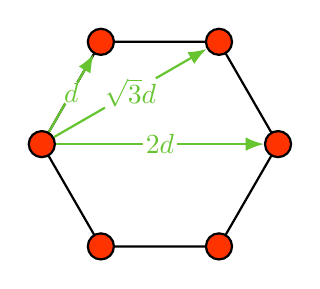
\begin{tikzpicture}[Benzene/.style={draw,thick, circle, radius = .1em,                                      fill=red!80!yellow},
                    arrow/.style={->, >=Latex,thick, yellow!40!green},
                    arrow_label/.style={midway, circle, fill=white, inner sep=0}
                    ]
        \newdimen\R
        \R=1.5cm
        \draw[thick] (0:\R)
        \foreach \x in {60,120,...,360} {  -- (\x:\R) }
        -- cycle (360:\R) node[Benzene] (Bc3){}
        -- cycle (300:\R) node[Benzene] (Bc4){}
        -- cycle (240:\R) node[Benzene] (Bc5){}
        -- cycle (180:\R) node[Benzene] (Bc0){}
        -- cycle (120:\R) node[Benzene] (Bc1){}
        -- cycle  (60:\R) node[Benzene] (Bc2){};
        
        \draw[arrow] (Bc0) -- (Bc1) node[arrow_label] {$d$};
        \draw[arrow] (Bc0) -- (Bc2) node[arrow_label] {$\sqrt{3}d$};
        \draw[arrow] (Bc0) -- (Bc3) node[arrow_label] {$2d$};
    \end{tikzpicture}
    \caption{Interatomic distances in Benzene ($d=\SI{1.40}{\angstrom})$}
    \label{fig:benzene_distances}
\end{figure}

\subsection{Hopping amplitudes}
One problem with modelling the benzene ring as a chain is that we lose the orientation of the lines connecting two sites relative to the light pulse direction.
This leads to an inaccuracy in the angle dependent time dependence of the hoppings between the sites. However, by comparing the results with those of another group, where the orientation was taken into account, we saw only negligible differences in the results and thus choose to move forward with this model.
%\medskip
%lexicographical indexing no longer produces proper hopping signs... but as mentioned we ignore that for now
    %%%%%%%%%%%%%%%%%
    % PULSE ON LINE %
    %%%%%%%%%%%%%%%%%
    
\begin{figure}[!hbt]
    \centering
    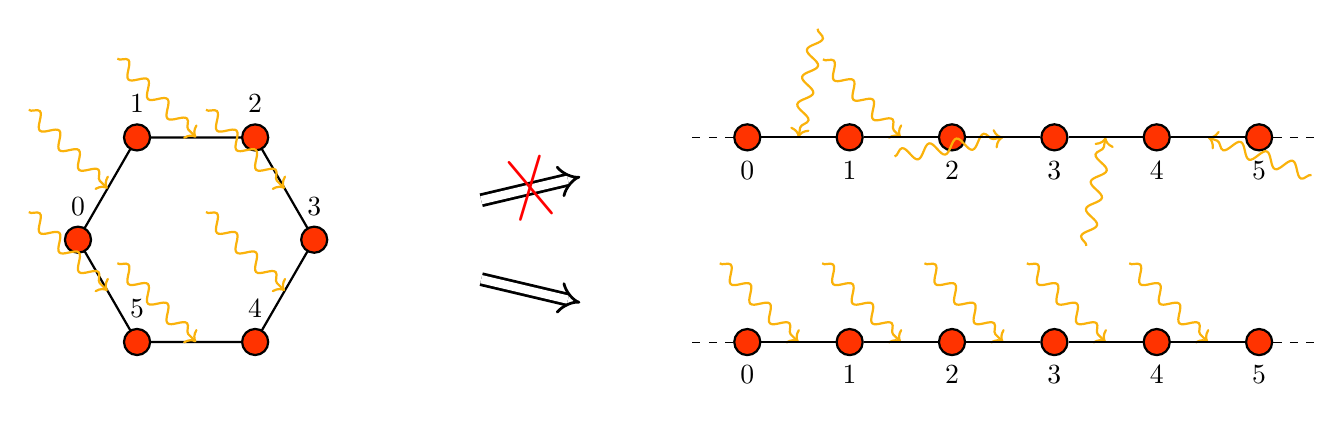
\begin{tikzpicture}[decoration=snake,
                    Benzene/.style={draw,thick, circle, radius = .1em, fill=red!80!yellow},
                    squiggly/.style={->, decorate, thick, yellow!70!red},
                    doublearrow/.style={->, double, line width=1pt, -Implies, double distance=3pt, shorten >= 2cm, shorten <=2cm}
                    ]
                    
    
    % RING %
    \newdimen\R
    \R=1.5cm
    \draw[thick] (0:\R)
    \foreach \x in {60,120,...,360} {  -- (\x:\R) }
    -- cycle (360:\R) node[Benzene, label=3] (Bc3){}
    -- cycle (300:\R) node[Benzene, label=4] (Bc4){}
    -- cycle (240:\R) node[Benzene, label=5] (Bc5){}
    -- cycle (180:\R) node[Benzene, label=0] (Bc0){}
    -- cycle (120:\R) node[Benzene, label=1] (Bc1){}
    -- cycle  (60:\R) node[Benzene, label=2] (Bc2){};
    
    \foreach \x/\y in {0/1,1/2,2/3,3/4,4/5,5/0}{
    \draw[squiggly] ($(Bc\x)!0.5!(Bc\y) + (-1,1)$) -- ($(Bc\x)!0.5!(Bc\y)$);
    }
    
    
    % CHAIN DOWN%
    \foreach \x in {0,1,2,3,4,5}
    \node[Benzene, label=below:\x] at ($(1.3*\x,0) + (7,-1.3)$)  (B\x){};
    
    \foreach \x/\y in {0/1, 1/2, 2/3, 3/4, 4/5}
    \draw[squiggly] ($(B\x)!0.5!(B\y) + (-1, 1)$) -- ($(B\x)!0.5!(B\y)$);
    
    \foreach \x/\y in {0/1,1/2,2/3,3/4,4/5}
    \draw[thick] (B\x) -- (B\y);
    
    \draw[dashed] ($(B0) - (0.7,0)$) -- (B0);
    \draw[dashed] (B5) -- ($(B5) + (0.7,0)$);
    
    % CHAIN UP %
    \foreach \x in {0,1,2,3,4,5}
    \node[Benzene, label=below:\x] at ($(1.3*\x,0) + (7,1.3)$)  (Bu\x){};
    
    \foreach \x/\y/\angle in {0/1/80, 1/2/135, 2/3/190, 3/4/260, 4/5/340}
    \draw[squiggly] ($(Bu\x)!0.5!(Bu\y) + (\angle:1.4)$) -- ($(Bu\x)!0.5!(Bu\y)$);

    \foreach \x/\y in {0/1,1/2,2/3,3/4,4/5}
    \draw[thick] (Bu\x) -- (Bu\y);

    \draw[dashed] ($(Bu0) - (0.7,0)$) -- (Bu0);
    \draw[dashed] (Bu5) -- ($(Bu5) + (0.7,0)$);
    

    % DOUBLE ARROWS %
    \draw[doublearrow] (Bc3) -- (Bu0) node[pos=0.5,sloped,rotate=150]{\color{red}\Huge$|$}node[pos=0.5,rotate=40]{\color{red}\Huge$|$};
    \draw[doublearrow] (Bc3) -- (B0);
    \end{tikzpicture}
    \caption{Caption}
\end{figure}
\section{Quantum Dot}

Quantum dots (QDs) are nanoscopic semiconducting particles that display interesting quantum mechanical effects. Due to their small size, the energy levels of the electrons within them become quantized, much like in atoms. Unlike atoms however, the size of QDs can be chosen arbitrarily, making their absorption spectra highly tunable.  Together with cost-effective manufacturing processes this makes QDs an enticing candidate for new photovoltaic technologies.
\medskip

Their high efficiency in energy conversion has been shown experimentally, and impact ionisation has been proposed as an explanation \cite{impact_io_in_qd}. In this work we first implement a quantum dot into our model, and investigate whether it can facilitate impact ionisation. Subsequently we couple the quantum dot to a larger molecule, benzene in this case, and investigate the effect of this on impact ionisation. This is motivated by the experimental work done in \cite{qd_motivation} where impact ionisation was seen in such a system.

\subsection{Geometry}
 
 In implementing quantum dots, one of two choices had to be made. Either we implement a new type of site, with multiple energy levels, or we model the quantum dot as a particular arrangement of sites, which we engineer to have the desired effective energy levels. The latter option requires less alterations to the existing code and thus was chosen.
 
 \medskip
 
 For all the computations done in this work the QD is modelled as a $2\times 2$ lattice of sites, with the following horizontal, vertical and diagonal hopping amplitudes: $v_h = v_v = 1$, $v_d = 0$.
 
 \medskip
 
 In order to be consistent with the model used for the Benzene ring, the nonlocal Coulomb interactions for the QD are also calculated using the PPP model as described in section \ref{subsec:ppp}. The distances used in the Ohno function, shown in Fig.
 \ref{fig:qd_distances}, were calculated by choosing the lattice constant to be equal to the $C-C$ bond length $d =\SI{1.4}{\angstrom}$. This does not necessarily have a physical basis, but for now it provides sufficient flexibility to engineer the desired spectrum by varying the on-site Coulomb interaction $U$, which is shown in section \ref{subsec:spectrum_engineering}.
 
\begin{figure}[!hbt]
    \begin{minipage}[b]{.48\textwidth}
        \centering
    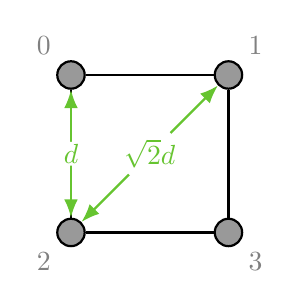
\begin{tikzpicture}[
                    QD/.style={draw,thick,circle, fill=black!40, inner sep=3.5},
                    QDlabel/.style={label={above left:{\color{gray}#1}}},
                    QDlabelRight/.style={label={above right:{\color{gray}#1}}},
                    arrow/.style={<->,>=Latex, thick, yellow!40!green},
                    arrow_label/.style={midway, circle, fill=white, inner sep=0}
                    ]
    \newdimen \qdd
    \qdd = 2cm
    %QD nodes    
    \node[QD, label={above left:{\color{gray}0}}]  at (0,\qdd)       (QD0){};
    \node[QD, label={above right:{\color{gray}1}}]  at (\qdd,\qdd)    (QD1){};
    \node[QD, label={below left:{\color{gray}2}}]   at (0,0)          (QD2){};
    \node[QD, label={below right:{\color{gray}3}}]  at (\qdd,0)       (QD3){};
    
    \draw[thick] (QD2.east) -- (QD3.west);
    \draw[thick] (QD0.east) -- (QD1.west);
    \draw[thick] (QD0.south) -- (QD2.north);
    \draw[thick] (QD1.south) -- (QD3.north);
    
    \draw[arrow] (QD2) -- (QD0) node[arrow_label] {$d$};
    \draw[arrow] (QD2) -- (QD1) node[arrow_label] {$\sqrt{2}d$};   
    
    \end{tikzpicture}
    
    \caption{Distances used in Ohno function (\ref{eq:ohno_interpolation}) to calculate the coulomb potential $U_{ij}$. With $d = \SI{1.4}{\angstrom}$\newline}
    \label{fig:qd_distances}
    \end{minipage}
    \hfill
    \begin{minipage}[b]{.48\textwidth}
        \centering
    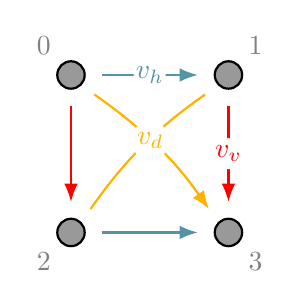
\begin{tikzpicture}[
                    QD/.style={draw,thick,circle, fill=black!40, inner sep=3.5},
                    QDlabel/.style={label={above left:{\color{gray}#1}}},
                    QDlabelRight/.style={label={above right:{\color{gray}#1}}},
                    arrow/.style={->, thick, yellow!40!green},
                    arrow_label/.style={midway, circle, fill=white, inner sep=0},
                    darrow_label/.style={pos=0.45, circle, fill=white, inner sep=1pt},
                    vhop/.style={->,>=Latex, thick, red, shorten <=0.2cm, shorten >=0.2cm},
                    hhop/.style={->,>=Latex, thick, cyan!70!red, shorten <=0.2cm, shorten >=0.2cm},
                    dhop/.style={->,>=Latex, thick, orange!60!yellow, shorten <=0.2cm, shorten >=0.2cm},
                    dhop2/.style={thick, orange!60!yellow, shorten <=0.2cm, shorten >=0.2cm}
                    ]
    \newdimen \qdd
    \qdd = 2cm
    %QD nodes    
    \node[QD, label={above left:{\color{gray}0}}]  at (0,\qdd)       (QD0){};
    \node[QD, label={above right:{\color{gray}1}}]  at (\qdd,\qdd)    (QD1){};
    \node[QD, label={below left:{\color{gray}2}}]   at (0,0)          (QD2){};
    \node[QD, label={below right:{\color{gray}3}}]  at (\qdd,0)       (QD3){};
    
    % vertical and horizonatal hoppings
    \draw[vhop] (QD1.south) --  (QD3.north) node[arrow_label] {$v_v$};
    \draw[vhop] (QD0.south) --  (QD2.north);
    \draw[hhop] (QD0.east)  --  (QD1.west)  node[arrow_label] {$v_h$};
    \draw[hhop] (QD2.east)  --  (QD3.west);
    
    % diagonal hoppings
    \draw[dhop2] (QD1.south west) to[out=215, in=55]                             (QD2.north east);
    \draw[dhop] (QD0.south east) to[out=-35, in=125] node[darrow_label] {$v_d$} (QD3.north west);
    
    
    \end{tikzpicture}
    \caption{Possible hoppings between QD sites. Arrow direction indicates the direction in which the sign of the imaginary part of the hopping amplitude is positive.}
    \label{fig:qd_hoppings}
    \end{minipage}
\end{figure}

 \subsection{Light pulse direction and hopping time dependence}
For every geometry, it is necessary to define a function that explicitly determines whether or not the hopping amplitude $v_{ij}$ between two any two sites $i$ and $j$ is time dependent, i.e. is modified by the light pulse.
\medskip

This depends on the direction of the light pulse, which for our implementation is always along the diagonal coming from the top left. Any hoppings perpendicular to the pulse direction will remain constant over time and are thus not time dependent.
\medskip

The sign of the imaginary parts of the hopping amplitudes is positive for hoppings parallel to the pulse direction and negative for hoppings perpendicular to the pulse direction. By labelling the sites in lexicographical order as shown in Fig. \ref{fig:qd_hoppings} we ensure that all hoppings from sites $i\to j$ have the same sign as $(j-i)$. The positive direction of the imaginary part of the hopping amplitudes are indicated in Fig. \ref{fig:qd_hoppings} by arrowheads. The diagonal hopping between sites 1 and 2 has no direction shown because in our case it is perpendicular to the light pulse and will have no effect anyway.


\section{Coupling QD-Benzene}
    The coupled QD-Benzene system is a combination of the above two systems with an extra hopping from all QD sites to a single Benzene site. Again the coulomb interactions are calculated via the Ohno interpolation and stored in the $U$ matrices. The distances used in the calculations for the $U$-matrix elements are shown in Fig. \ref{fig:coupled_distances}. The hopping amplitudes are the same as in the isolated systems with the addition of a parameter $v_c$, representing the hopping between the QD and the benzene ring. By setting $v_c = 0$ we would expect to see the same spectra as with the Isolated systems. It is important to note that as was alluded to in \ref{sec:electron_hole_symmetry} the on-site hopping term (chemical potential) $v_{ii}$ differs for Benzene and for QD sites and must thus be calculated separately. The hopping matrix is shown in Fig. \ref{fig:coupled_hoppings}
    \medskip
    
    For now we only investigate how the system responds to the light pulse only interacting with the QD sites. Thus we set all the benzene hoppings and the hoppings between the QD and benzene to be non-time dependent.

\begin{itemize}
    \item {\color{red} why would we expect to see impact ionisation in such a coupled system? previous papers?}
\end{itemize}

\usetikzlibrary{matrix, positioning}

\colorlet{mgreen}{green!80!black!30}
\colorlet{myellow}{yellow!90!red!70}
\newcommand{\my}{|[fill=myellow]|}
\renewcommand{\mg}{|[fill=mgreen]|}



\begin{figure}[!hbt]
    \centering
    \begin{tikzpicture}[cell/.style={rectangle,draw=black},
                    space/.style={minimum height=1.5em,matrix of nodes,row sep=-\pgflinewidth,column sep=-\pgflinewidth},
                    text depth=0.5ex,text height=2ex,nodes in empty cells,
                    headers/.style={font=\footnotesize, color=blue!60!black!30},
                    QD/.style={draw,thick,circle, radius = .1em, fill=black!40, inner sep=0},
                    Benzene/.style={draw,thick, circle, radius = .1em, fill=red!80!yellow, inner sep=0},
                    nlabelcolor/.style={gray},
                    QDlabel/.style={label={above left:{\color{gray}#1}}}
                    ]
    
    %maybe use brace to indicate Benzene and QD regions https://texample.net/tikz/examples/model-physics/
    \matrix (first) [space,nodes={cell,minimum width=2em, minimum height=2em}]
    {
    \my         & 1             & 1         & $\sqrt{2}$& \mg -     & -         & -         & -         & -         & -        \\
    1           & \my           & $\sqrt{2}$& 1         & \mg -     & -         & -         & -         & -         & -        \\
    1           & $\sqrt{2}$    & \my       & 1         & \mg -     & -         & -         & -         & -         & -        \\
    $\sqrt{2}$  & 1             & 1         & \my       & \mg -     & -         & -         & -         & -         & -        \\
    \mg -       & \mg -         & \mg -     & \mg -     & \my       & 1         & $\sqrt{3}$& 2         & $\sqrt{3}$& 1        \\
    -           & -             & -         & -        & 1         &  \my      & 1         & $\sqrt{3}$& 2         & $\sqrt{3}$ \\
    -           & -             & -         & -         & $\sqrt{3}$& 1         & \my       & 1         & $\sqrt{3}$& 2        \\
    -           & -             & -         & -         & 2         & $\sqrt{3}$& 1         &  \my      & 1         & $\sqrt{3}$ \\
    -           & -             & -         & -         & $\sqrt{3}$& 2         & $\sqrt{3}$& 1         & \my       & 1        \\
    -           & -             & -         & -         & 1         & $\sqrt{3}$& 2         & $\sqrt{3}$& 1         &  \my \\ };
    
    \foreach \i/\x in {0/1, 1/2,2/3,3/4,4/5,5/6, 6/7, 7/8, 8/9, 9/10}{
    \node[headers, anchor=north] at ([yshift=4ex]first-1-\x.north) {\i};
    \node[headers, anchor=west] at ([xshift=-4ex]first-\x-1.west) {\i};
    }
    %%%%%%%%%%%%%%%%%%%%%%%%%%%%%%%%%%%%%%%%%%%
    %%%%%%%%%%%%%%%%%%%%%%%%%%%%%%%%%%%%%%%%%%%
    \tikzset{shift={(6,1)}}
    \newdimen \qdd
    \qdd = 2cm
    %QD nodes    
    \node[QD, QDlabel={2}] at (0,0)          (QD2){};
    \node[QD, QDlabel={3}] at (\qdd,0)       (QD3){};
    \node[QD, QDlabel={0}] at (0,\qdd)       (QD0){};
    \node[QD, QDlabel={1}] at (\qdd,\qdd)    (QD1){};
    
    \draw[thick] (QD2.east) -- (QD3.west);
    \draw[thick] (QD0.east) -- (QD1.west);
    \draw[thick] (QD0.south) -- (QD2.north);
    \draw[thick] (QD1.south) -- (QD3.north);
    
    
    %Benzene Nodes
    \newdimen\R
    \R=1.5cm
    \tikzset{shift={(5,1)}}
    \draw[thick] (0:\R)
    \foreach \x in {60,120,...,360} {  -- (\x:\R) }
    -- cycle (360:\R) node[Benzene, label={[nlabelcolor]7}] (B7){}
    -- cycle (300:\R) node[Benzene, label={[nlabelcolor]8}] (B8){}
    -- cycle (240:\R) node[Benzene, label={[nlabelcolor]9}] (B9){}
    -- cycle (180:\R) node[Benzene, label={[nlabelcolor]4}] (B4){}
    -- cycle (120:\R) node[Benzene, label={[nlabelcolor]5}] (B5){}
    -- cycle  (60:\R) node[Benzene, label={[nlabelcolor]6}] (B6){};
    
    
    \tikzset{shift={(0,0)}}
    \foreach \x in {3, 1} \draw[color=red, thick] (QD\x.east) to [out=0, in=180] (B4.west);
    \draw[color=red, thick] (QD2.south) to [out = 270, in=180] (B4.west);
    \draw[color=red, thick] (QD0.north) to [out = 90, in=180] (B4.west);
    
    
    %%%%%%%%%%%%%%%%%%%%%%%%%%%%%%
    %%%%%%%%%%%%%%%%%%%%%%%%%%%%%%%
    % LEGEND
    
    \node [draw, rectangle, fill=myellow, minimum size=1em, inner sep=0, label={[align=left, text width=170pt]right: $\begin{cases} - &\text{ for equal spin matrix} \\ 1 &\text{ for opposite spin matrix}\end{cases}$}] at ($(QD2) + (0, -1.6)$) {};
    
    \node [draw, rectangle, fill=mgreen, minimum size=1em, inner sep=0, label={[align=left, text width=170pt]right: We assume strong shielding between benzene and quantum dot $\Rightarrow$ no Coulomb interaction}] at ($(QD2) + (0, -3.)$) {-};
    
    
    \end{tikzpicture}
    \caption{Table showing the structure of the coulomb interaction matrices $U_{ij\sigma\sigma'}$. Each entry represents the distance between two sites as a multiple of the C-C bond length $d=\SI{1.40}{\angstrom}$. The $U_{ij}$ matrices can be constructed by applying the Ohno function \ref{eq:ohno_interpolation} to each entry in the table. Note that a dash implies an infinite distance (- $= \infty$).}
    \label{fig:coupled_distances}
\end{figure}


%%%%%%%%%%%%%%%%%%%%%%%%%%%%%%%
%%%%%%%%%%%%%%%%%%%%%%%%%%%%%%%

\newcommand{\viiQD}   {|[fill=green!59]| $v_{ii}^{\text{qd}}$}
\newcommand{\viiBZ}   {|[fill=green!40]| $v_{ii}^{\text{b}}$}
\newcommand{\vh}    {|[fill=red!30]| $v_h$}
\newcommand{\vv}    {|[fill=yellow!80!red!50]| $v_v$}
\newcommand{\vd}    {|[fill=pink!50]| $v_d$}
\newcommand{\vc}    {|[fill=cyan!80!blue!20]| $v_c$}

\begin{figure}[!hbt]
    \centering
    \begin{tikzpicture}[cell/.style={rectangle,draw=black},
                    space/.style={minimum height=1.5em,matrix of nodes,row sep=-\pgflinewidth,column sep=-\pgflinewidth},
                    text depth=0.5ex,text height=2ex,nodes in empty cells,
                    headers/.style={font=\footnotesize, color=blue!60!black!30},
                    QD/.style={draw,thick,circle, radius = .1em, fill=green!80!yellow, inner sep=0},
                    Benzene/.style={draw,thick, circle, radius = .1em, fill=red!80!yellow, inner sep=0},
                    nlabelcolor/.style={gray},
                    QDlabel/.style={label={above left:{\color{gray}#1}}}
                    ]

    \matrix (first) [space,nodes={cell,minimum width=2.3em, minimum height=2.3em}]
    {
    \viiQD  & \vh   & \vv   & \vd  & \vc  & 0    & 0    & 0    & 0    & 0    \\
    \vh     & \viiQD& \vd   & \vv  & \vc  & 0    & 0    & 0    & 0    & 0    \\
    \vv     & \vd   & \viiQD& \vh  & \vc  & 0    & 0    & 0    & 0    & 0    \\
    \vd     & \vv   & \vh   & \viiQD & \vc  & 0    & 0    & 0    & 0    & 0    \\
    \vc     & \vc   & \vc   & \vc  & \viiBZ & \vh  & 0    & 0    & 0    & \vh  \\
    0       & 0     & 0     & 0    & \vh  & \viiBZ & \vh  & 0    & 0    & 0    \\
    0       & 0     & 0     & 0    & 0    & \vh  & \viiBZ & \vh  & 0    & 0    \\
    0       & 0     & 0     & 0    & 0    & 0    & \vh  & \viiBZ & \vh  & 0    \\
    0       & 0     & 0     & 0    & 0    & 0    & 0    & \vh  & \viiBZ & \vh  \\
    0       & 0     & 0     & 0    & \vh  & 0    & 0    & 0    & \vh  & \viiBZ \\ };
    
    \foreach \i/\x in {0/1, 1/2,2/3,3/4,4/5,5/6, 6/7, 7/8, 8/9, 9/10}{
    \node[headers, anchor=north] at ([yshift=4ex]first-1-\x.north) {\i};
    \node[headers, anchor=west] at ([xshift=-4ex]first-\x-1.west) {\i};
    }
    \end{tikzpicture}
    \caption{Table shows distances between sites, as multiples of the C-C bond length ($d=\SI{1.40}{\angstrom}$) {\color{red} idk maybe add functions on how to generate table... prbly not nescessary though}}
    \label{fig:coupled_hoppings}
\end{figure}

%
\chapter{Results}
\section{Isolated Quantum Dot}
\subsection{Engineering the spectrum}
\begin{itemize}
    \item $vd= 0$
\end{itemize}

\begin{figure}[!hbt]
    \centering
    \includegraphics[width=0.7\textwidth]{graph/spectrum_engineering.pdf}
    \caption{temporary. Lehmann spectrum taken on site 0, but looks the same on all sites. if it matters black to white transition can be improved}
\end{figure}

\subsection{Not seeing transition at expected energie}
\section{Isolated Benzene}
    In order to verify if our new implementations work as intended, we compare the spectral functions we obtain for the isolated benzene ring with the one obtained by F. Hörbinger via exact diagonalisation of the PPP model \cite{hoerbinger}. We find that our results shown in Fig. \ref{fig:isolated_benzene} match those from \cite{hoerbinger} up to three significant figures, after conversion into the appropriate units. Thus we can be fairly confident that our implementation works, at least for the isolated Benzene system.

\medskip
\begin{figure}[!hbt]
    \centering
    \includegraphics[width=0.7\textwidth]{graph/isolated_benzene.pdf}
    \caption{Spectral function of isolated benzene with peak energies in agreement with results from \cite{hoerbinger}\newline
    Parameters: $U = 3.96$, $a = 0.3$, $t_0 = 0$, broadening-factor $\epsilon = 0.1 $
    }\label{fig:isolated_benzene}
\end{figure}

Additionally we can also see from Fig. \ref{fig:isolated_benzene} that both the Lehmann spectrum and the spectral function obtained via the Fourier transformation of the Green's function produce comparable results, the only differences being the ``noise" that is introduced in the Greens function spectrum due to the Fourier transform. This could be suppressed further by tweaking the broadening factor and the zero-padding of the domain, as briefly described in \ref{sec:spectral_functions}.
\section{Coupled System}

\subsection{Testing}
Before we investigate the effects of increasing the coupling strength between the two systems, we verify that if the hopping amplitude $v_c = 0$, the spectra on the individual sites remain unchanged. For the coupled system, calculating the Lehmann spectrum is no longer an option as memory becomes a limiting factor, instead we resort to using the Green's function method.

\medskip
As can be seen when comparing Fig. \ref{fig:coupled_vc_0} with the spectra in Fig. \ref{fig:spectrum_engineering} and Fig. \ref{fig:isolated_benzene}, this is indeed the case. The slight variations being due to a difference in parameters used to perform the Fourier transformation.

\begin{figure}[!hbt]
    \centering
    \includegraphics[width=0.49\textwidth]{graph/coupled_QD_vc_0.pdf}
    \includegraphics[width=0.49\textwidth]{graph/coupled_benzene_vc_0.pdf}sh
    \caption{Spectral function of all the sites of the coupled system with the coupling parameter turned off, $v_c = 0$. These spectra should be identical to those in Fig. \ref{fig:spectrum_engineering} and Fig. \ref{fig:isolated_benzene}}
    \label{fig:coupled_vc_0}
\end{figure}

\subsection{Dependence of the spectrum on the coupling strength}

\begin{figure}[!hbt]
    \centering
    \includegraphics[width=0.49\textwidth]{graph/spectrum_vc_sweep/QD_All_020.pdf}
    \includegraphics[width=0.49\textwidth]{graph/spectrum_vc_sweep/QD_All_030.pdf}
    \includegraphics[width=0.49\textwidth]{graph/spectrum_vc_sweep/QD_All_070.pdf}
    \includegraphics[width=0.49\textwidth]{graph/spectrum_vc_sweep/QD_All_100.pdf}
    \caption{}
    \label{fig:spectrum_vc_sweep}
\end{figure}
\newpage
 1. Introduction to this topic
    - keep it short (1-2pages)
    - reference Hörbinger + original PPP papers
    - Innerberger
    
 2. Code that I implemented
    - non-local interaction
    - potential energy (instead of double occupancy)... double occupancy not a good measure of pot energy anymore
    - vii (Hubbard term)

3. Results
    - Greens functions
    - show QD and Benzene isolated (compare to PPP paper)
    - show coupled QD and Benzene (with vc = 0 and with vc != 0)
    
4. Outlook
    - this was about the setup
    - next work is about analysing this system (impact ionisation on BzRing or QD)
    - why no transitions as w=4 (maybe some k point stuff)
    
What the reader should get from the thesis
1.(How the new implemented code works and how one can use it)
2.(How does a spectrum of QD to Benzene ring look)

\newpage

\bibliographystyle{unsrt} % https://www.overleaf.com/learn/latex/Bibtex_bibliography_styles
\bibliography{bibliography.bib} 

\newpage
% inspo for code diagram https://texample.net/tikz/examples/tcp-state-machine/

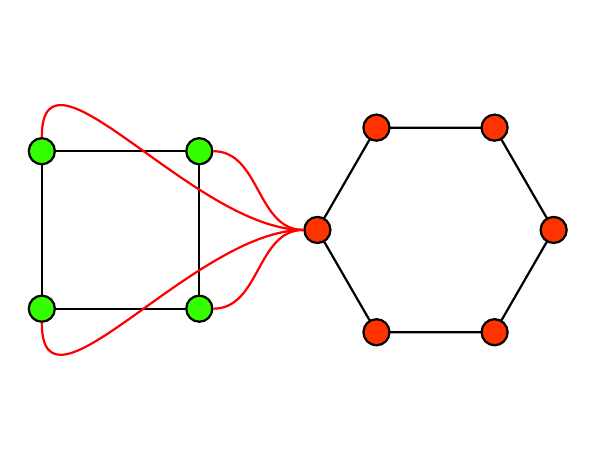
\begin{tikzpicture}[%
    QD/.style={draw,thick,circle, radius = .1em, fill=green!80!yellow},
    Benzene/.style={draw,thick, circle, radius = .1em, fill=red!80!yellow}
    ]
    
    \newdimen \qdd
    \qdd = 2cm
    %QD nodes    
    \node[QD] at (0,0)          (QD0){};
    \node[QD] at (\qdd,0)       (QD1){};
    \node[QD] at (0,\qdd)       (QD2){};
    \node[QD] at (\qdd,\qdd)    (QD3){};
    
    \draw[thick] (QD0.east) -- (QD1.west);
    \draw[thick] (QD2.east) -- (QD3.west);
    \draw[thick] (QD2.south) -- (QD0.north);
    \draw[thick] (QD3.south) -- (QD1.north);
    
    
    %Benzene Nodes
    \newdimen\R
    \R=1.5cm
    \tikzset{shift={(5,1)}}
    \draw[thick] (0:\R)
    \foreach \x in {60,120,...,360} {  -- (\x:\R) }
    -- cycle (360:\R) node[Benzene] (B0){}
    -- cycle (300:\R) node[Benzene] (B1){}
    -- cycle (240:\R) node[Benzene] (B2){}
    -- cycle (180:\R) node[Benzene] (B3){}
    -- cycle (120:\R) node[Benzene] (B4){}
    -- cycle  (60:\R) node[Benzene] (B5){};
    
    \tikzset{shift={(0,0)}}
    \foreach \x in {1, 3} \draw[color=red, thick] (QD\x.east) to [out=0, in=180] (B3.west);
    \draw[color=red, thick] (QD0.south) to [out = 270, in=180] (B3.west);
    \draw[color=red, thick] (QD2.north) to [out = 90, in=180] (B3.west);
\end{tikzpicture}

\vskip 5cm
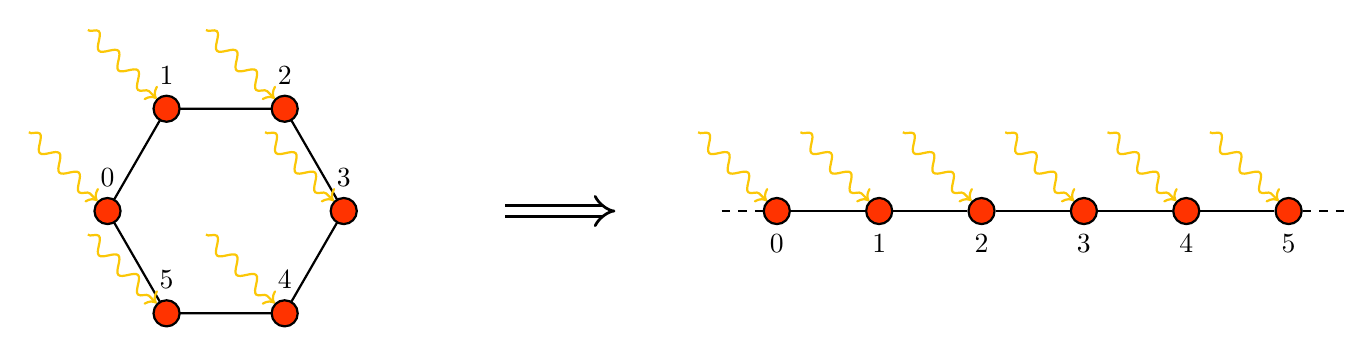
\begin{tikzpicture}[decoration=snake,
                    Benzene/.style={draw,thick, circle, radius = .1em, fill=red!80!yellow}
                    ]
    % RING %
    \newdimen\R
    \R=1.5cm
    \draw[thick] (0:\R)
    \foreach \x in {60,120,...,360} {  -- (\x:\R) }
    -- cycle (360:\R) node[Benzene, label=3] (Bc3){}
    -- cycle (300:\R) node[Benzene, label=4] (Bc4){}
    -- cycle (240:\R) node[Benzene, label=5] (Bc5){}
    -- cycle (180:\R) node[Benzene, label=0] (Bc0){}
    -- cycle (120:\R) node[Benzene, label=1] (Bc1){}
    -- cycle  (60:\R) node[Benzene, label=2] (Bc2){};
    
    \foreach \x in {0,1,2,3,4,5}{
    \draw[->, decorate, thick, yellow!80!red] ($(Bc\x) + (-1, 1)$) -- (Bc\x);
    }
    
    % CHAIN %
    \foreach \x in {0,1,2,3,4,5}{
    \node[Benzene, label=below:\x] at ($(1.3*\x,0) + (7,0)$)  (B\x){};
    \draw[->, decorate, thick, yellow!80!red] ($(B\x) + (-1, 1)$) -- (B\x);
    }
    
    \draw[dashed] ($(B0) - (0.7,0)$) -- (B0);
    \draw[thick] (B0) -- (B1);
    \draw[thick] (B1) -- (B2);
    \draw[thick] (B2) -- (B3);
    \draw[thick] (B3) -- (B4);
    \draw[thick] (B4) -- (B5);
    \draw[dashed] (B5) -- ($(B5) + (0.7,0)$);

    % MIDDLE ARROW %
    \node[] at ($(Bc3)!0.5!(B0)$) (mid){};
    \draw[->, double, line width=1pt, -Implies, double distance=3pt] ($(mid) - (0.7,0)$) -- ($(mid) + (0.7,0)$);
    
    \end{tikzpicture}
\end{document}